% -----------------------------------------------------------------------------
% Sugestão de inserção no seu cap_3.tex ou onde desejar apresentar os resultados
% -----------------------------------------------------------------------------

Para a execução da simulação, foi desenvolvido o \textit{script} em linguagem Python, cuja rotina completa de amostragem, verificação lógica e cálculo de erros iterativos é apresentada a seguir:

\begin{verbatim}
import random
import math
import matplotlib.pyplot as plt

def estimar_pi_monte_carlo(N):
    acertos = 0

    # Listas para armazenar o histórico e gerar os gráficos depois
    historico_pi = []
    erros_absolutos = []
    erros_relativos_percentuais = []
    pontos_x_dentro, pontos_y_dentro = [], []
    pontos_x_fora, pontos_y_fora = [], []

    pi_anterior = 0  # Inicialização para o cálculo do erro iterativo

    for k in range(1, N + 1):  # k vai de 1 até N
        # Gerar coordenadas x, y uniformemente distribuídas entre 0 e 1 
        x = random.random()
        y = random.random()

        # Verifica se o ponto está dentro do círculo
        if x * x + y * y <= 1:
            acertos += 1
            # Salvando para o gráfico de dispersão 
            if N <= 10000:
                pontos_x_dentro.append(x)
                pontos_y_dentro.append(y)
        else:
            if N <= 10000:
                pontos_x_fora.append(x)
                pontos_y_fora.append(y)

        # Calcula a estimativa atual de pi
        pi_k = 4 * (acertos / k)
        historico_pi.append(pi_k)
        
        
        # Cálculo dos erros iterativos (comparando com o passo anterior)
        if k > 1:
            Ea = abs(pi_k - pi_anterior)
            Er = Ea / abs(pi_k) if pi_k != 0 else 0
            Erp = Er * 100
        else:
            Ea, Er, Erp = 0, 0, 0

        erros_absolutos.append(Ea)
        erros_relativos_percentuais.append(Erp)

        pi_anterior = pi_k

    # Análise de Erro Final em relação ao valor verdadeiro de Pi (math.pi)
    pi_estimado_final = historico_pi[-1]
    erro_abs_real = abs(pi_estimado_final - math.pi)
    erro_rel_perc_real = (erro_abs_real / math.pi) * 100

    print(f"--- Resultados para N = {N} ---")
    print(f"Pi Estimado: {pi_estimado_final:.5f}")
    print(f"Pi Real (math.pi): {math.pi:.5f}")
    print(f"Erro Absoluto (Real): {erro_abs_real:.5f}")
    print(f"Erro Relativo Percentual (Real): {erro_rel_perc_real:.5f}%")

    # --- Geração de Gráficos  ---
    if N <= 10000: 
        plt.figure(figsize=(12, 5))

        # Gráfico 1: Distribuição dos pontos
        plt.subplot(1, 2, 1)
        plt.scatter(pontos_x_dentro, pontos_y_dentro, color='blue',
        s=1, label='Dentro')
        plt.scatter(pontos_x_fora, pontos_y_fora, color='red',
        s=1, label='Fora')
        plt.title('Distribuição dos Pontos (Monte Carlo)')
        plt.xlabel('x')
        plt.ylabel('y')
        plt.legend()
        plt.axis('equal')

        # Gráfico 2: Convergência de Pi
        plt.subplot(1, 2, 2)
        plt.plot(range(1, N + 1), historico_pi, label='Pi Estimado',
        color='purple')
        plt.axhline(y=math.pi, color='green', linestyle='--',
        label='Pi Verdadeiro')
        plt.title('Convergência da Estimativa de Pi')
        plt.xlabel('Número de Iterações (k)')
        plt.ylabel('Valor de Pi')
        plt.legend()

        plt.tight_layout()
        plt.show()


# Executando a simulação
estimar_pi_monte_carlo(N=10000)
\end{verbatim}

A compilação do código para $N = 10000$ amostras permitiu a tabulação dos dados de convergência iterativa e a extração do comportamento estocástico dos dardos simulados. Os resultados gráficos desta iteração estão expostos na \autoref{fig:grafico_monte_carlo}.

\begin{figure}[htb]
    \caption{\label{fig:grafico_monte_carlo}Distribuição dos pontos e convergência da estimativa de Pi.}
    \begin{center}
        % Substitua "nome_da_sua_imagem_salva.png" pelo arquivo gerado pelo seu código
        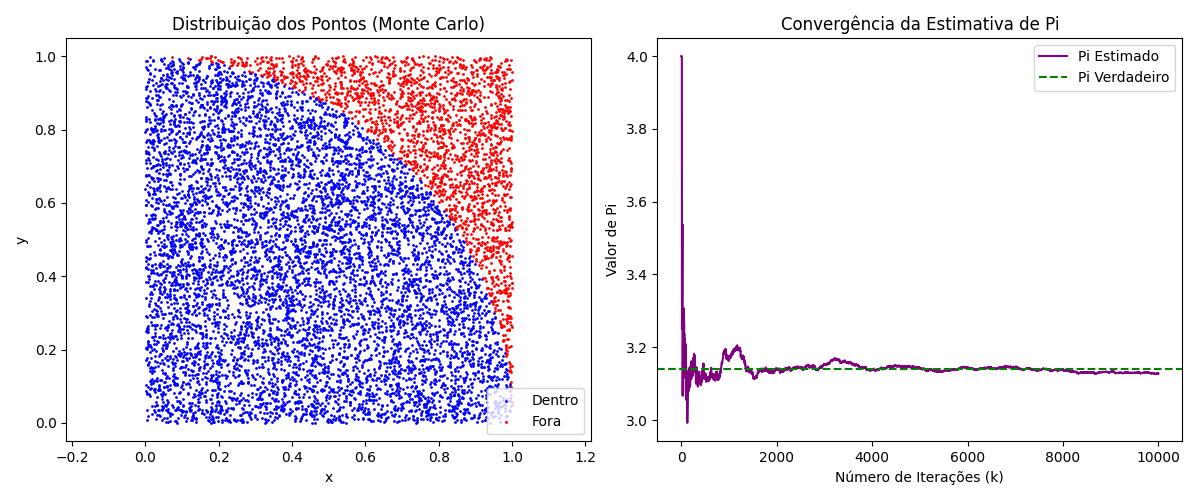
\includegraphics[width=1.0\textwidth]{figuras/grafico_montecarlo.png}
    \end{center}
    \fonte{Elaborado pelo autor (2026).}
\end{figure}
A execução do algoritmo matemático para uma amostragem de $N = 10.000$ iterações produziu os resultados quantitativos sintetizados na \autoref{tab:resultados_n10000}.

\begin{table}[htb]
    \centering
    \ABNTEXfontereduzida
    \caption{\label{tab:resultados_n10000}Resultados da estimativa de Pi para N = 10.000.}
    \begin{tabular}{@{}lc@{}}
        \toprule
        \textbf{Métrica Analisada} & \textbf{Valor Obtido} \\ \midrule
        Valor de \texorpdfstring{$\pi$}{pi} Estimado & 3,12760 \\
        Valor de \texorpdfstring{$\pi$}{pi} Real (\texttt{math.pi}) & 3,14159 \\
        Erro Absoluto ($E_a$) & 0,01399 \\
        Erro Relativo Percentual ($E_{rp}$) & 0,44540\% \\ \bottomrule
    \end{tabular}
    \fonte{Elaborado pelo autor (2026).}
\end{table}

A partir dos dados da \autoref{tab:resultados_n10000}, constata-se que, mesmo com um número inicial conservador de amostras ($N = 10.000$), o modelo apresentou um erro relativo percentual inferior a 0,5\%. Isso confirma que o erro absoluto ($E_a = 0,01399$) já se encontra na escala dos centésimos, validando a eficácia e a coerência teórica do estimador estocástico.